\documentclass[12pt, a4paper, oneside, titlepage, portrait]{report}

\usepackage{ngerman}
\usepackage[utf8]{inputenc}
\usepackage[T1]{fontenc}
\usepackage{latexsym}
\usepackage{amsmath,amsfonts,amssymb,amsthm,amscd}
\usepackage{dsfont}
\usepackage{graphicx}
\usepackage[flushleft]{paralist} 
\usepackage[dvipsnames]{xcolor} 
\usepackage[all]{xy}
\usepackage{makeidx}
\usepackage{graphicx}
\usepackage{verbatim}
\usepackage[numbers]{natbib} % [numbers,round]

\usepackage{pgf}
\usepackage{tikz}
\usepackage{pgfplots}
\usepackage{mathrsfs}
\usepackage{adjustbox}
\usepackage{float}
\usepackage[margin=1in]{geometry}

% \usepackage{showframe}

\usetikzlibrary{arrows}
\pgfplotsset{compat=1.15}
 \pagenumbering{gobble}
\begin{document}
		\begin{adjustbox}{center}
			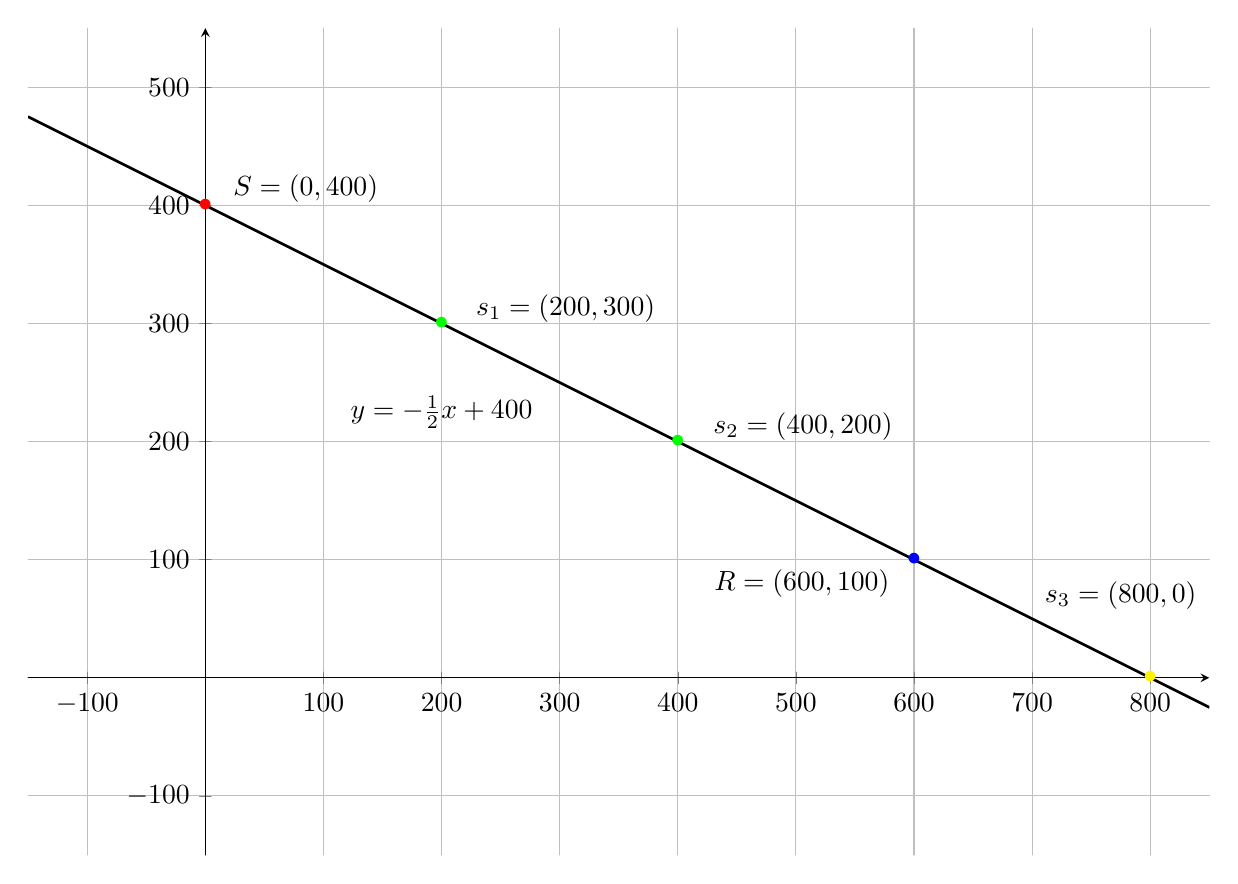
\begin{tikzpicture}[line cap=round,line join=round,>=triangle 45,x=0.015cm,y=0.015cm]
				\begin{axis}[x=0.015cm,y=0.015cm,axis lines=middle,ymajorgrids=true,xmajorgrids=true,
				xmin=-150.,xmax=850.,xtick={-100.,0.,...,850.},
				ymin=-150.,ymax=550.,ytick={-100.,0.,...,550.},]
				\clip(-150.,-150.) rectangle (850.,550.);
				\draw [line width=1.pt,domain=-150.:850.] plot(\x,{(--240000.-300.*\x)/600.});
				\draw (200.,225.) node {$y=-\frac{1}{2}x+400$};
				\draw[color=red] (0.,400.) node {$ \bullet $};
				\draw (85.,414.) node {$S=(0,400)$};
				\draw[color=blue] (600.,100.) node {$ \bullet $};
				\draw (505.,80.) node {$R=(600,100)$};
				\draw[color=green] (200.,300.) node {$ \bullet $};
				\draw (305.,313.) node {$s_1=(200,300)$};
				\draw[color=green] (400.,200.) node {$ \bullet $};
				\draw (506.,213.) node {$s_2=(400,200)$};
				\draw[color=yellow] (800.,0.) node {$ \bullet $};
				\draw (775.,70.) node {$s_3=(800,0)$};
				\end{axis}
			\end{tikzpicture}
		\end{adjustbox}\\\\\\\\\\\\\\
		\begin{adjustbox}{center}
			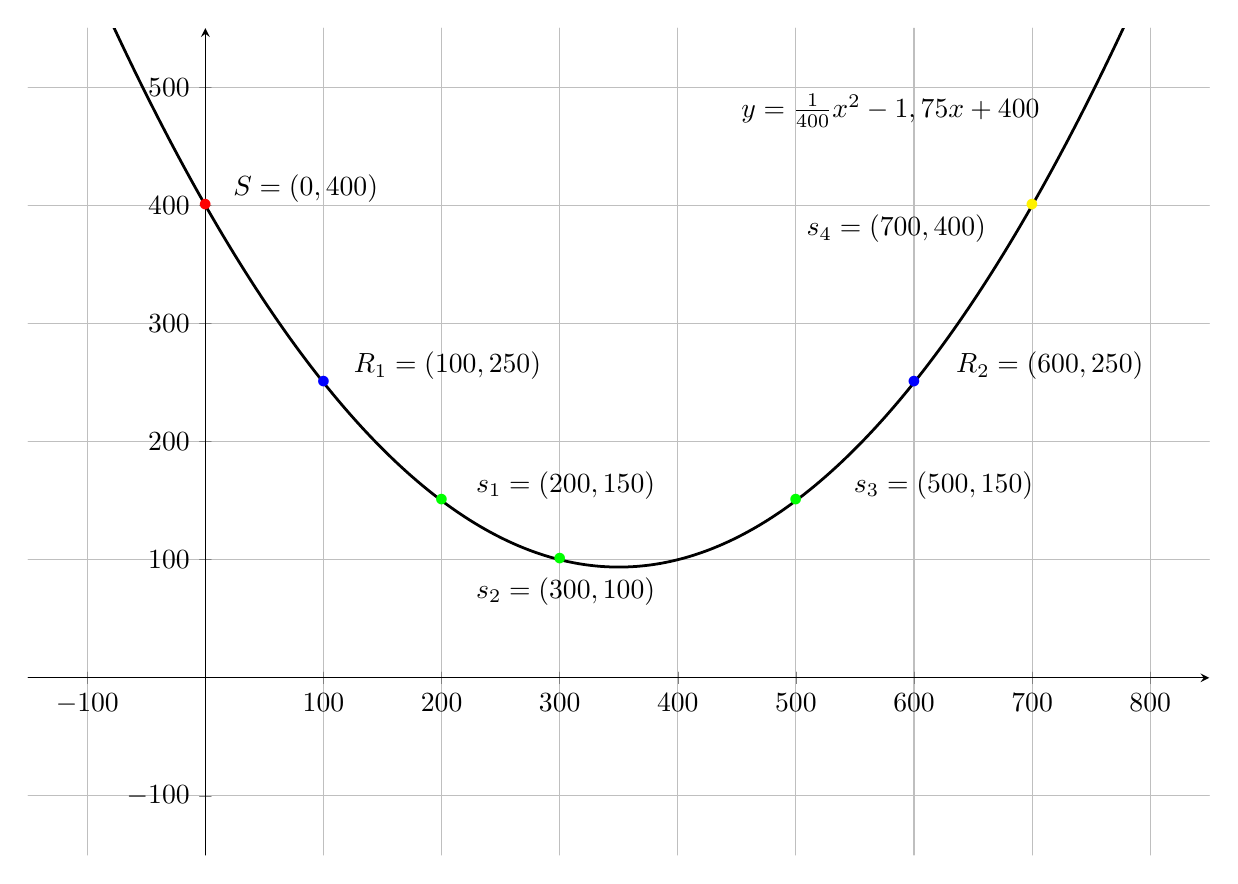
\begin{tikzpicture}[line cap=round,line join=round,>=triangle 45,x=0.015cm,y=0.015cm]
			\begin{axis}[x=0.015cm,y=0.015cm,axis lines=middle,ymajorgrids=true,xmajorgrids=true,
			xmin=-150.,xmax=850.,xtick={-100.,0.,...,850.},
			ymin=-150.,ymax=550.,ytick={-100.,0.,...,550.},]
			\clip(-150.,-150.) rectangle (850.,550.);
			\draw[line width=1.pt,smooth,samples=100,domain=-150.0:850.0] plot(\x,{0.0025*(\x)^(2.0)-1.75*(\x)+400.0});
			\draw[color=red] (0.,400.) node {$ \bullet $};
			\draw (85.,414.) node {$S=(0,400)$};
			\draw[color=blue] (100.,250.) node {$ \bullet $};
			\draw (205.,264.) node {$R_1=(100,250)$};
			\draw[color=blue] (600.,250.) node {$ \bullet $};
			\draw (715.,264.) node {$R_2=(600,250)$};
			\draw (580.,480.) node {$y=\frac{1}{400}x^2-1,75x+400$};
			\draw[color=green] (200.,150.) node {$ \bullet $};
			\draw (305.,163.) node {$s_1=(200,150)$};
			\draw[color=green] (300.,100.) node {$ \bullet $};
			\draw (305.,73.) node {$s_2=(300,100)$};
			\draw[color=green] (500.,150.) node {$ \bullet $};
			\draw (625.,163.) node {$s_3=(500,150)$};
			\draw[color=yellow] (700.,400.) node {$ \bullet $};
			\draw (585.,380.) node {$s_4=(700,400)$};
			\end{axis}
			\end{tikzpicture}
		\end{adjustbox}
\end{document}
